
%File: anonymous-submission-latex-2025.tex
\documentclass[letterpaper]{article} % DO NOT CHANGE THIS
% \usepackage[submission]{aaai25}  % DO NOT CHANGE THIS
\usepackage{aaai25}  % DO NOT CHANGE THIS
\usepackage{times}  % DO NOT CHANGE THIS
\usepackage{helvet}  % DO NOT CHANGE THIS
\usepackage{courier}  % DO NOT CHANGE THIS
\usepackage[hyphens]{url}  % DO NOT CHANGE THIS
\usepackage{graphicx} % DO NOT CHANGE THIS
\urlstyle{rm} % DO NOT CHANGE THIS
\def\UrlFont{\rm}  % DO NOT CHANGE THIS
\usepackage{natbib}  % DO NOT CHANGE THIS AND DO NOT ADD ANY OPTIONS TO IT
\usepackage{caption} % DO NOT CHANGE THIS AND DO NOT ADD ANY OPTIONS TO IT
\frenchspacing  % DO NOT CHANGE THIS
\setlength{\pdfpagewidth}{8.5in} % DO NOT CHANGE THIS
\setlength{\pdfpageheight}{11in} % DO NOT CHANGE THIS
\usepackage{boldline,multirow,booktabs, subfig}
\newcommand{\shortname}{LAMA-UT}
% These are recommended to typeset algorithms but not required. See the subsubsection on algorithms. Remove them if you don't have algorithms in your paper.
\usepackage{algorithm}
\usepackage{algorithmic}
\usepackage{pgfplots}
\pgfplotsset{compat=1.18}


%
% These are are recommended to typeset listings but not required. See the subsubsection on listing. Remove this block if you don't have listings in your paper.
\usepackage{newfloat}
\usepackage{listings}
\DeclareCaptionStyle{ruled}{labelfont=normalfont,labelsep=colon,strut=off} % DO NOT CHANGE THIS
\lstset{%
	basicstyle={\footnotesize\ttfamily},% footnotesize acceptable for monospace
	numbers=left,numberstyle=\footnotesize,xleftmargin=2em,% show line numbers, remove this entire line if you don't want the numbers.
	aboveskip=0pt,belowskip=0pt,%
	showstringspaces=false,tabsize=2,breaklines=true}
\floatstyle{ruled}
\newfloat{listing}{tb}{lst}{}
\floatname{listing}{Listing}
%
% Keep the \pdfinfo as shown here. There's no need
% for you to add the /Title and /Author tags.
\pdfinfo{
/TemplateVersion (2025.1)
}

% DISALLOWED PACKAGES
% \usepackage{authblk} -- This package is specifically forbidden
% \usepackage{balance} -- This package is specifically forbidden
% \usepackage{color (if used in text)
% \usepackage{CJK} -- This package is specifically forbidden
% \usepackage{float} -- This package is specifically forbidden
% \usepackage{flushend} -- This package is specifically forbidden
% \usepackage{fontenc} -- This package is specifically forbidden
% \usepackage{fullpage} -- This package is specifically forbidden
% \usepackage{geometry} -- This package is specifically forbidden
% \usepackage{grffile} -- This package is specifically forbidden
% \usepackage{hyperref} -- This package is specifically forbidden
% \usepackage{navigator} -- This package is specifically forbidden
% (or any other package that embeds links such as navigator or hyperref)
% \indentfirst} -- This package is specifically forbidden
% \layout} -- This package is specifically forbidden
% \multicol} -- This package is specifically forbidden
% \nameref} -- This package is specifically forbidden
% \usepackage{savetrees} -- This package is specifically forbidden
% \usepackage{setspace} -- This package is specifically forbidden
% \usepackage{stfloats} -- This package is specifically forbidden
% \usepackage{tabu} -- This package is specifically forbidden
% \usepackage{titlesec} -- This package is specifically forbidden
% \usepackage{tocbibind} -- This package is specifically forbidden
% \usepackage{ulem} -- This package is specifically forbidden
% \usepackage{wrapfig} -- This package is specifically forbidden
% DISALLOWED COMMANDS
% \nocopyright -- Your paper will not be published if you use this command
% \addtolength -- This command may not be used
% \balance -- This command may not be used
% \baselinestretch -- Your paper will not be published if you use this command
% \clearpage -- No page breaks of any kind may be used for the final version of your paper
% \columnsep -- This command may not be used
% \newpage -- No page breaks of any kind may be used for the final version of your paper
% \pagebreak -- No page breaks of any kind may be used for the final version of your paperr
% \pagestyle -- This command may not be used
% \tiny -- This is not an acceptable font size.
% \vspace{- -- No negative value may be used in proximity of a caption, figure, table, section, subsection, subsubsection, or reference
% \vskip{- -- No negative value may be used to alter spacing above or below a caption, figure, table, section, subsection, subsubsection, or reference

\setcounter{secnumdepth}{0} %May be changed to 1 or 2 if section numbers are desired.

% The file aaai25.sty is the style file for AAAI Press
% proceedings, working notes, and technical reports.
%

% Title

% Your title must be in mixed case, not sentence case.
% That means all verbs (including short verbs like be, is, using,and go),
% nouns, adverbs, adjectives should be capitalized, including both words in hyphenated terms, while
% articles, conjunctions, and prepositions are lower case unless they
% directly follow a colon or long dash
\title{LAMA-UT: Language Agnostic Multilingual ASR through Orthography Unification and Language-Specific Transliteration}
\author{
    %Authors
    % All authors must be in the same font size and format.
    Sangmin Lee\textsuperscript{\rm 1},
    Woojin Chung\textsuperscript{\rm 1},
    Hong-Goo Kang\textsuperscript{\rm 1}\thanks{Corresponding author}\\
}
\affiliations{
    %Afiliations
    \textsuperscript{\rm 1}Dept. of Electrical \& Electronic Engineering, Yonsei University, South Korea\\
    \{sangmin\_lee, woojinchung\}@dsp.yonsei.ac.kr, hgkang@yonsei.ac.kr
}

\begin{document}

\maketitle

\begin{abstract}

Building a universal multilingual automatic speech recognition (ASR) model that performs equitably across languages has long been a challenge due to its inherent difficulties.
To address this task we introduce a \textbf{L}anguage-\textbf{A}gnostic \textbf{M}ultilingual \textbf{A}SR pipeline through orthography \textbf{U}nification and language-specific \textbf{T}ransliteration (\shortname\footnote{Codes: https://github.com/sanghyang00/lama-ut}).
\shortname~operates without any language-specific modules while matching the performance of state-of-the-art models trained on a minimal amount of data.
Our pipeline consists of two key steps.
First, we utilize a universal transcription generator to unify orthographic features into Romanized form and capture common phonetic characteristics across diverse languages. 
Second, we utilize a universal converter to transform these universal transcriptions into language-specific ones.
In experiments, we demonstrate the effectiveness of our proposed method leveraging universal transcriptions for massively multilingual ASR.
Our pipeline achieves a relative error reduction rate of 45\% when compared to Whisper and performs comparably to MMS, despite being trained on only 0.1\% of Whisper's training data.
Furthermore, our pipeline does not rely on any language-specific modules.
However, it performs on par with zero-shot ASR approaches which utilize additional language-specific lexicons and language models.
We expect this framework to serve as a cornerstone for flexible multilingual ASR systems that are generalizable even to unseen languages.

\end{abstract}
\section{Introduction}

Developing a model for multilingual automatic speech recognition (ASR) is appealing due to its applicability to universal languages, including low-resource or unseen languages.
However, this task presents significant challenges as it requires extensive datasets and involves the complexity of capturing shared characteristics across diverse languages in both phonetic and orthographic domains.

Since the revolution in ASR technologies driven by self-supervised learning (SSL) models~\cite{NEURIPS2020_92d1e1eb, conneau2020unsupervisedcrosslingualrepresentationlearning, hsu2021hubert, chen2022wavlm}, monolingual ASR has achieved superhuman transcription performance, shifting the main focus of recent research towards developing a universal model that spans multiple languages.

There are two primary methods for building a multilingual ASR model.
The first approach involves scaling the size of both the labeled dataset and the model itself, using a single universal model to enhance its capacity and cover a vast number (100+) of languages, thereby achieving multilingual ASR~\cite{radford2023robust}.
Another approach involves incorporating language-specific modules into the universal model to address the performance inconsistencies of previous methods. 
For example, MMS~\cite {JMLR:v25:23-1318} demonstrated the feasibility of scaling multilingual technology to over 1,000 languages by leveraging common features across languages and adding language-specific modules to improve the performance of each language.
Indeed, there have been efforts to integrate both methods~\cite{zhang2023googleusmscalingautomatic}, combining their strengths to build a more robust and versatile model.

Although these works have demonstrated strong performance across various languages, the trade-off between performance and complexity remains a substantial challenge.
The first method, using a single universal pipeline, struggles to achieve consistent performance across languages, and its effectiveness in low-resource languages remains uncertain.
On the other hand, despite achieving state-of-the-art performance and parameter efficiency, the second method cannot be considered a single universal model due to the inclusion of language-specific modules. Moreover, the use of language-specific modules like adapters, heads, and language models (LMs) sometimes complicates the training and inference pipeline, suggesting potential areas for future improvement.
\begin{figure*}[]
    \centering
    \includegraphics[width=\textwidth]{figures/pipeline.png}
    \caption{Illustration of our universal ASR pipeline.}
    \label{fig:pipeline}
\end{figure*}

Simultaneously, large language models (LLMs) have garnered considerable attention for their remarkable capabilities in the natural language processing (NLP) domain.
Following this trend, ASR pipelines have integrated audio SSL models as encoders and LLMs as decoders to enhance transcription quality~\cite{li2023prompting, fathullah2024prompting}.
These approaches involve using projectors~\cite{yu2024connecting} or fine-tuning strategies~\cite{tang2024salmonn, du2024lauragptlistenattendunderstand} to align modalities and improve transcription capabilities across multilingual datasets.
Subsequently, shallow fusion~\cite{chorowski2016betterdecodinglanguagemodel, kannan2018analysis} based scoring methods~\cite{hu2023massively, huang2024multilingual} were attempted to replace conventional LMs with LLMs during the decoding stage.
Despite these efforts resulting in performance gain across various languages, a comprehensive method to fully leverage the diverse emergent abilities of LLMs remains to be developed.

In this paper, we introduce a novel language-agnostic multilingual ASR pipeline that spans over 100 languages, including completely unseen languages. 
As in Fig~\ref{fig:pipeline}, the proposed pipeline consists of two phases: universal transcription generation and language-specific transliteration.
In the universal transcription generation phase, we focused on reducing orthographic complexity by unifying diverse orthographic systems into a consistent format, approximating phonetic features across multiple languages.
In the language-specific transliteration phase, we regard the transformation from universal transcription to language-specific transcription as a transliteration task by leveraging a universal converter.
Our experiments demonstrate notable transcription performance of~\shortname~across over 100 languages while using significantly smaller training data (only 680 hours) compared to other state-of-the-art multilingual ASR models.
Furthermore, our proposed pipeline outperforms previous methods, especially in low-resource languages, and demonstrates proficiency in completely unseen languages, achieving performance comparable to existing language-agnostic ASR methods without relying on any language-specific modules.
Our contributions are summarized as follows:

\begin{itemize}
    \item We propose a novel language-agnostic multilingual ASR pipeline consisting of two phases: universal transcription generation and language-specific transliteration.
    \item We enabled our proposed pipeline to perform multilingual ASR with minimal data by unifying diverse orthographic systems through Romanization.
    \item Our pipeline demonstrates consistent performance across over 100 seen languages and excels with completely unseen languages, all without relying on any language-specific modules or additional fine-tuning.
    
\end{itemize}
\section{Related Works}
\subsection{Multilingual ASR}
Initially, multilingual ASR models handled a limited number of languages~\cite{toshniwal2018multilingual, pratap2020massivelymultilingualasr50}, under 60. 
However, recent advancements have led to the development of models capable of managing a broader range of languages.
Whisper~\cite{radford2023robust} uses a sequence-to-sequence~\cite{NIPS2014_a14ac55a} approach with 680,000 hours of weakly supervised data, and its neural decoder serves as a LM, enhancing transcription performance.
With this method, Whisper attained impressive performance across most supported languages.

Google USM~\cite{zhang2023googleusmscalingautomatic} employs a Conformer~\cite{gulati20_interspeech} encoder with various types of heads~\cite{graves2012sequencetransductionrecurrentneural, chan2016listen} and is trained on an extensive dataset. 
It also employs a three-stage training incorporating speech-only, speech-text paired, and text-only data. 
Furthermore, to enhance transcription performance for low-resource languages, USM integrates language-specific adapters and employs Noisy Student Training (NST) techniques~\cite{9156610, Park_2020}. 

MMS~\cite{JMLR:v25:23-1318}, a state-of-the-art multilingual ASR model, employed a Connectionist Temporal Classification (CTC) based approach~\cite{graves2006connectionist} on a dataset covering over 1,000 languages. 
It utilizes a two-stage fine-tuning pipeline.
The first stage involves Romanization-based fine-tuning to learn a global representation across diverse languages. 
In the second stage, language-specific adapters and heads are added to capture detailed features for each language and fine-tuned.

\subsection{Zero-Shot ASR}
ASR-2K~\cite{li22aa_interspeech} is a zero-shot ASR model which utilizes three universal models to cover a range of languages: an acoustic model~\cite{li2020universal}, a pronunciation model~\cite{li2022zero}, and a LM~\cite{scannell12007crubadan}.
This suggests the potential for a universal multilingual ASR model capable of functioning in a zero-shot environment without relying on any language-specific components.
Consequently, Zero-Shot MMS~\cite{zhao2024scalingsimpleapproachzeroshot} utilized language-specific lexicon and n-gram LMs in the decoding phase to enhance zero-shot transcription performance. 

\subsection{LLM-Supported Multilingual ASR}
\citealt{hu2023massively} trained a multilingual LLM covering 84 languages and employed a shallow fusion-based per-frame scoring to enhance transcription quality in multilingual ASR.
Subsequently,~\citealt{huang2024multilingual} introduced non-autoregressive per-segment scoring, which improves transcription performance and reduces the computational burden.
These methods primarily leveraged the strengths of a multilingual acoustic model (USM) and achieved further accuracy by incorporating LLMs into the decoding step.
\section{Proposed Method}
The overall structure of the proposed multilingual ASR pipeline,~\shortname, comprises a universal transcription generation phase and a language-specific transliteration phase, as shown in Fig~\ref{fig:pipeline}. 
We produce universal transcriptions by finetuning an audio encoder with an additional classification layer.
Consequently, we manually select a prompt type from a predefined dictionary and combine it with language information to generate the input prompt for the universal converter.
Finally, by feeding this input prompt into the universal converter, we translate the universal transcription into language-specific ones.

\subsection{Universal Transcription Generation}
Previous studies in linguistics~\cite{ladefoged1996sounds, clark2007introduction} have shown that the phonological characteristics of human speech are constrained by a limited range of sounds due to the anatomical structure of the vocal tract. 
Similarly, in the ASR domain, prior research~\cite{taguchi-chiang-2024-language} has empirically demonstrated that the primary obstacle in multilingual ASR is the orthographic complexity across languages.
Through the integration of these two insights, we aim to unify orthographic systems across diverse languages by standardization of notations into a Latin character system.
This approach establishes alignment between phonetic and orthographic features through a unified transcription system.
As a result, we develop a universal transcription generator capable of producing consistent transcriptions across multilingual speech corpora, including unseen languages. 

\subsubsection{International Phonetic Alphabet.} 
The first method for orthography unification is to use the international phonetic alphabet (IPA).
IPA is a phonetic notation system that includes four elements: consonants, vowels, diacritics, and suprasegmentals. 
IPA can precisely transcribe pronunciations in a consistent format with a combination of the four elements.
There are challenges with the IPA, especially in vocabulary mapping, and one possible solution is to treat the combination of elements as a single token (e.g., ts, dz, etc.).
However, due to the vast diversity of possible combinations makes this approach difficult to implement.
Conversely, treating each IPA character as a distinct token introduces another issue: characters without phonetic value must be mapped to specific frames as shown in Fig~\ref{fig:problems}.
Since diacritics and suprasegmentals provide detailed information about pronunciation (e.g., length, tone, and stress) but do not carry specific phonetic values, mapping them to distinct frames can introduce confusion during the training process. 

\begin{table*}[h!]
\centering
\small
\begin{tabular}{l||l}
\toprule
\textbf{Zero-Shot}                                                                  & Transcribe following Romanized sentence into a \{lang\} sentence: \{roman\}.                                                                                                                                                                                                 \\ \midrule
\textbf{Few-Shot}                                                                   & \begin{tabular}[l]{@{}l@{}}Here are some examples of transcribing a Romanized sentence into a \{lang\} sentence: \{shots\}.\\Considering the examples above, transcribe the following Romanized sentence into a \{lang\} sentence: \{roman\}.\end{tabular}                     \\ \midrule
\textbf{Zero-Shot CoT}                                                              & Transcribe the following Romanized sentence into a \{lang\} sentence. Think step by step: \{roman\}.                                                                                                                                                                            \\ \midrule
\textbf{\begin{tabular}[l]{@{}l@{}}Few-Shot +\\ Zero-Shot CoT\end{tabular} }        & \begin{tabular}[l]{@{}l@{}}Here are some examples of transcribing a Romanized sentence into a \{lang\} sentence: \{shots\}.\\Considering the examples above, transcribe the following Romanized sentence into a \{lang\} sentence. \\Think step by step: \{roman\}.\end{tabular} \\ \midrule

\textbf{\multirow{2}{*}{\begin{tabular}[l]{@{}l@{}}Prompt\\Chaining\end{tabular}}} & \begin{tabular}[l]{@{}l@{}}Transcribe the following Romanized sentence into a \{lang\} sentence, based on its pronunciation: \{roman\}.\end{tabular}\\ \cmidrule{2-2} & \begin{tabular}[l]{@{}l@{}}Correct the typographical and spacing errors in the following \{lang\} sentence: \{pred\}.\end{tabular}     \\ \bottomrule                                 
\end{tabular}%
\caption{Specific format of the prompt. \textit{roman} refers to the predicted Romanized transcription, \textit{shots} indicates generated examples sampled from the training data, \textit{pred} denotes output from first prompt and \textit{lang} indicates the name of the language.}
\label{prompt_example_tab}
\end{table*}
\subsubsection{Romanization.} Romanization is an alternative method for orthography unification which involves converting text from various writing systems into Latin script.
While Romanization does not preserve phonetic features as precisely as the IPA, it generally retains phonetic information.
Additionally, Romanization offers several advantages over the IPA.
Romanization standardizes diverse writing systems using the Latin alphabet, which is already employed by the majority of languages.
In contrast, IPA requires a specific set of rules for converting the orthography of each language into its IPA representation.
Thus, Romanization is more efficient as it only requires conversion for languages that do not use the Latin alphabet.
Furthermore, Romanization is advantageous for LLMs, as a large portion of their training data consists of Latin characters.
Given these benefits, we adopt Romanization as a method for orthography unification. 

\begin{figure}[]
    \centering
    \includegraphics[width=\columnwidth]{figures/problems.png}
    \caption{Problems derived in single-token IPA recognition. Diacritic `:' indicates phoneme length, which has no explicit phonetic value. $\epsilon$ denotes a blank token in CTC.}
    \label{fig:problems}
\end{figure}
\subsubsection{Universal Transcription Generator.} 
Since our goal is to generate a universal transcription with unified orthography, our first approach was leveraging a wav2vec2.0-phoneme~\cite{xu2021simpleeffectivezeroshotcrosslingual}.
However, we found that directly passing phoneme tokens to the universal converter is suboptimal for transliteration, as it generates phoneme-level tokens without accounting for spacing. 
To address this, we shifted our focus to developing a universal transcription generator that produces character-level tokens while incorporating spacing information.
In this context, Romanization provides a universal character-level orthographic representation, effectively reducing the vocabulary size to around 30 tokens compared to IPA.
Since Romanization aligns with the common phonetic features preserved across languages, we are also confident in the proposed method's strong generalization ability for languages not explicitly included in the training data.
We selected wav2vec2.0-XLS-R~\cite{babu2021xlsrselfsupervisedcrosslingualspeech} with 1 billion parameters, an SSL model pre-trained on 128 languages, as the audio encoder to leverage the advantages of pre-training on a diverse set of languages.
We then attach a classification layer on top and fine-tune both the audio encoder and the classification layer with speech and Romanized transcription pairs to generate universal transcriptions.

\subsection{Language-Specific Transliteration}
The next step is to revert the universal transcription, which retains phonetic features, back to its original language-specific form. 
Since this process involves a text-to-text transformation, we approach it as a transliteration task.
Consequently, we focused on the versatility of LLMs which excel in multilingual and multitask benchmarks due to extensive training on diverse text data.
Therefore, we aim to utilize LLMs as universal converters to transform Romanized transcriptions into language-specific ones.

\subsubsection{Prompt Generation.}
While LLMs have brought a tectonic shift to the NLP domain, additional techniques are still needed to fully harness their emergent abilities.
In this context, prompt engineering has emerged as a field focused on crafting and refining prompts to effectively utilize LLMs across diverse applications and research areas.
To maximize the performance of the inversion process, in the ablation study, we empirically investigated various prompt types: zero-shot, few-shot, zero-shot chain-of-thought (CoT), and prompt chaining, to determine which is the most appropriate for this task. 

\subsubsection{Universal Converter.}
We transliterate the unified Romanized transcription by leveraging LLM's multilingual and multitask language understanding ability without finetuning.
Since our approach does not require any special fine-tuning, the universal converter can be replaced with any superior LLMs, potentially improving the performance of our proposed pipeline in line with the rapidly advancing capabilities of LLMs.
For this paper implementation, we utilize LLaMA3-8B, 4-bit quantized LLaMA3-70B~\cite{touvron2023llamaopenefficientfoundation}, and GPT-4o-mini~\cite{openai2024gpt4technicalreport} as the universal converter.

\section{Experiments}
\subsection{Dataset}
\subsubsection{FLEURS.} FLEURS~\cite{conneau2022fleursfewshotlearningevaluation} is a multilingual speech corpus encompassing 102 languages. It provides a relatively small amount of data per language (approximately 12 hours) while ensuring an unbiased distribution of data across the languages.
Given our focus on demonstrating effective multilingual ASR with minimal data, we utilize the FLEURS and its official splits for experiments.
\subsubsection{CommonVoice.} CommonVoice~\cite{ardila-etal-2020-common} is a multilingual speech dataset crowdsourced from speakers of various languages. For unseen languages, we leverage the official test split of 25 languages from CommonVoice 17.0, which offers sufficient samples for evaluation.

\subsection{Data Preprocessing}
We initially applied NFKC normalization and lowercase transformation to the text transcriptions. 
Subsequently, we excluded samples containing parentheses or numbers from the dataset for the following reasons:
parentheses and digits in transcriptions introduced ambiguity, as some enclosed phrases were pronounced while others were not, and digits had one-to-many pronunciation mappings across languages (e.g. `1' can be pronounced as `one', `eins', `uno', `yi', etc.).
Finally, we utilized the Python library \textit{Uroman}~\cite{hermjakob-etal-2018-box} to obtain Romanized transcription and \textit{Phonemizer}~\cite{Bernard2021} for IPA transcription.
For Japanese, we employed \textit{Pykakasi}~\cite{takahashi1992kakasi} due to the limitation of \textit{Uroman}, which treats Japanese kanji as Chinese characters.
Following these preprocessing steps, we obtained approximately 6 to 8 hours of speech-transcription paired data per language on average.

\begin{table*}[t]
\centering
\small
\begin{tabular}{l||ccccccc|cccc}
\toprule
\multirow{2}{*}{Model}                                                                    & \multicolumn{7}{c|}{Seen (PER / CER $\downarrow$)}                                   & \multicolumn{4}{c}{Unseen (PER / CER $\downarrow$)}                    \\ %\cline{2-12} 
                                                                                          & de & nl  & fr  & es  & it  & \multicolumn{1}{c|}{pt}  & avg  & ia    & eo    & \multicolumn{1}{c|}{eu}    & avg \\ \midrule \midrule
\multirow{2}{*}{\begin{tabular}[c]{@{}l@{}}wav2vec2.0-phoneme\textsuperscript{\dag}\\ + n-gram LM\textsuperscript{\dag}\end{tabular}} & 23.8 & 38.0 & 31.0 & 28.7 & 33.5 & \multicolumn{1}{c|}{45.0} & 33.0 & 10.7 & - & \multicolumn{1}{c|}{20.8} & 31.4   \\
                                                                                          & 14.8 & 26.0  & 26.4  & 12.3    & 21.7    & \multicolumn{1}{c|}{36.5}    & 22.9    & \textbf{6.1}    & -    & \multicolumn{1}{c|}{\textbf{13.7}}    & \textbf{22.2}   \\ \midrule
IPA generator (\shortname)                                                                      & 10.2  & 10.5 & \textbf{9.6} & \textbf{4.2} & 4.6 & \multicolumn{1}{c|}{10.9} & 14.4 & 29.0 & 32.0 & \multicolumn{1}{c|}{36.6} & 35.1  \\ 
\textbf{Roman generator (\shortname)}                                                                    & \textbf{7.3}  & \textbf{9.6} & 12.9 & 4.4 & \textbf{3.6} & \multicolumn{1}{c|}{\textbf{7.2}} & \textbf{11.3} & 14.0 & \textbf{20.8} & \multicolumn{1}{c|}{30.3} & 32.3  \\ \bottomrule
\end{tabular}%
\caption{
Comparison between two orthography unification methods. We report PER and CER for seen and unseen languages. 
Average values are calculated over all 102 seen and 25 unseen languages, respectively. For a fair comparison, all the model sizes are set to 300 million. $\dagger$ denotes results measured by PER, which does not allow for a strict comparison with other results. The language codes and their corresponding language names are provided in the appendix.}
\label{orthography_comp_tab}
\end{table*}
\begin{table}[]
\centering
\small
\begin{tabular}{c|ccc}
\toprule
Model    & \begin{tabular}[c]{@{}c@{}}Data (h)\end{tabular}& \begin{tabular}[c]{@{}c@{}}Universal\end{tabular}  & \begin{tabular}[c]{@{}c@{}}Zero-Shot\end{tabular} \\ 
\midrule\midrule
Whisper & 680k & O &  X \\
MMS-1162   & 122k    & X & X \\
\textbf{\shortname}  &  \textbf{0.6k} & \textbf{O} & \textbf{O} \\ \bottomrule 
\end{tabular}%
\caption{Comparison of previous multi-lingual ASR models with the proposed pipeline. \textit{Data} denotes the total amount of training dataset, \textit{Universal} indicates that no language-specific module is needed, and \textit{Zero-Shot} denotes whether inference on unseen languages is feasible.}
\label{brief_comp_tab}
\end{table}
\subsection{Training Detail}
We performed fine-tuning on all layers except the feature extractor for 3,000 steps with a CTC loss and a batch size of 128.
We bypassed the two-stage fine-tuning pipeline from prior studies~\cite{xu2021simpleeffectivezeroshotcrosslingual, JMLR:v25:23-1318} because our distinct methodology, which used a smaller dataset, caused the divided fine-tuning approach to result in premature convergence and instability.
For hyperparameters, we employed the default AdamW optimizer~\cite{kingma2017adammethodstochasticoptimization, loshchilov2018decoupled} with a tri-stage learning rate scheduler. The warm-up, hold, and decay phases were configured to 10\%, 60\%, and 30\% of the total training steps, respectively.
We then performed a series of experiments to determine the optimal learning rate schedule within the range of 5e-6 to 5e-4.
Finally, the entire training pipeline was conducted on two RTX-3090 GPUs with 24GB of VRAM each, and we leveraged gradient accumulation techniques to address memory issues.

\subsection{Inference Detail}
\subsubsection{Universal Transcription Generator.} 
We leveraged a beam search decoder from flashlight~\cite{kahn2022flashlight} with a beam size of 100. 
No additional lexicons or LMs were utilized in the decoding pipeline to maintain a universal pipeline without relying on language-specific elements.

\subsubsection{Prompting Strategy.}
For the prompting strategy, we utilized language information and a subset of the training data to construct our hypothesis prompt. The specific format of the prompt employed is detailed in Table~\ref{prompt_example_tab}.
In zero-shot prompting, the universal converter automatically transforms Romanized transcriptions into language-specific ones using only the Romanized transcriptions and language information. We employed zero-shot prompting to evaluate the performance of the LLM with minimal input.
Few-shot prompting~\cite{NEURIPS2020_1457c0d6} involves providing examples to help the model generate responses to subsequent instances. 
We hypothesized that this approach would be particularly effective for low-resource or unseen languages by inducing in-context learning. 
Specifically, we randomly sampled five Romanized transcription and target transcription pairs for each few-shot example.
Zero-shot CoT prompting~\cite{NEURIPS2022_8bb0d291} is a technique that supports complex reasoning by inducing the decomposition of intricate tasks into detailed steps. 
Specifically, we appended the phrase ``Let's think step by step'' to the input prompt to encourage the reasoning of the model.
Prompt chaining employs a sequence of prompts, with each prompt building upon the output of the previous one, to manage complex multi-step tasks.
In this aspect, we concentrated on the decomposable process of converting predicted Romanized transcriptions into language-specific transcriptions through \textit{(i) reverse-Romanization} and \textit{(ii) error correction}.
We considered that errors in Romanized transcriptions could propagate during transliteration to language-specific ones, potentially reducing system performance.

\begin{table}[!t]
\centering
\small
\begin{tabular}{c|ccc}
\toprule
                        & Universal Converter       & CER $\downarrow$  & WER $\downarrow$  \\ \midrule\midrule
\multirow{3}{*}{Seen}   & LLaMA-8B    & 26.6 & 46.7 \\
                        & LLaMA-70B   & 15.5 & 35.3 \\
                        & \textbf{GPT-4o-mini} & \textbf{7.5}  & \textbf{18.1} \\ \midrule
\multirow{3}{*}{Unseen} & LLaMA-8B    & 33.0 & 50.2 \\
                        & LLaMA-70B   & 27.2 & 58.9 \\
                        & \textbf{GPT-4o-mini} & \textbf{15.8} & \textbf{38.3} \\ \bottomrule
\end{tabular}%
\caption{
Upper bound performance of the universal converter. 
This upper bound is assessed by feeding ground truth Romanized transcriptions into the universal converter with zero-shot prompting.}
\label{upper_bound_tab}
\end{table}
\subsubsection{Universal Converter.}
Finally, we required the output of the universal converter to conform to a specific format.
We instruct the model to enclose the output within three backticks (e.g., \texttt{```}), which allows us to isolate and sort only the language-specific transcription from the output of the model.
We set the temperature value to 0.0 for all LLMs to obtain deterministic results.
\begin{table*}[]
\centering
\small
\begin{tabular}{c|c||rrr|rrr|rrr}
\toprule
\multirow{2}{*}{Resource} & \multirow{2}{*}{Lang.} & \multicolumn{3}{c|}{Whisper-large-v3}            & \multicolumn{3}{c|}{MMS-1162}                    & \multicolumn{3}{c}{\shortname}   \\ 
                          &                           &Data (h) &CER $\downarrow$  &WER $\downarrow$  &Data (h) &CER $\downarrow$ &WER $\downarrow$ &Data (h) &CER $\downarrow$  &WER $\downarrow$ \\ \midrule\midrule
\multirow{3}{*}{High}     & es                   & 11000            & 1.2  & 3.1  &        2969          &  1.6   &  5.8   & \textbf{6.1}              & 2.8  & 7.3  \\
                          & it                   & 2585             & 0.5  & 1.6  &     1566             &  1.2   &  5.2   & \textbf{6.8}              & 2.0  & 5.2  \\
                          & id                & 1014             & 1.4  & 5.7  &      71            &  2.9   &  14.2   & \textbf{6.8}              & 4.2  & 11.5 \\ \midrule
\multirow{3}{*}{Middle}   & ta                     & 136              & 18.3 & 26.7 &         265         &  11.0   &  41.5   & \textbf{6.3}              & 19.5 & 31.9 \\
                          & ur                      & 104              & 30.9 & 65.0 &      57            &  9.0   &  29.0   & \textbf{4.9}              & 14.9 & 31.9 \\
                          & sk                    & 90               & 2.9  & 8.7  &      301            &  2.2   &  8.8   & \textbf{4.5}              & 3.8  & 10.2 \\ \midrule
\multirow{3}{*}{Low}      & mk                & 16               & 10.3 & 26.3 &       45           &   1.5  &  8.1   & \textbf{5.1}              & 5.5  & 17.2 \\
                          & hi                     & 12               & 35.9 & 43.3 &      57            &  5.8  &   19.6  & \textbf{5.0}              & 8.2  & 15.0 \\ 
                          & kk                   & 12               & 8.5  & 35.1 &         46         &  2.8   &  15.2   & \textbf{8.1}              & 6.7  & 22.9 \\\midrule\midrule
\multicolumn{2}{c||}{Average}                   & -                & 23.9 & 42.9 &         -         &  \textbf{7.8}   &  \textbf{28.8}   & -                & \textbf{14.8} & \textbf{33.2} \\ \bottomrule
\end{tabular}%
\caption{
Comparison results with the baseline models.
Average CER and WER have reported over 82 languages from FLEURS that are covered by Whisper, MMS, and our method. 
The classification of the amount of resources is based on the volume of training data used by Whisper. 
We utilized MMS which encompasses 1162 languages, trained on a combined dataset from MMS-lab, FLEURS, CommonVoice, Voxpopuli~\cite{wang-etal-2021-voxpopuli}, and MLS~\cite{Pratap_2020}.} 
\label{baseline_comparison_tab}
\end{table*}
\begin{figure*}[ht]
    \centering
    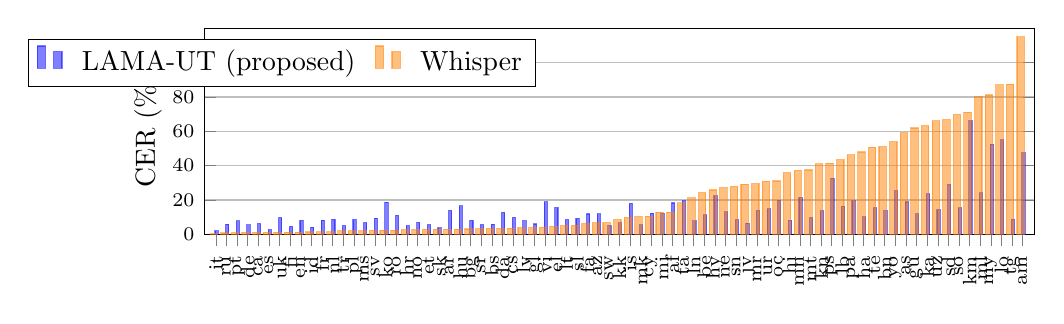
\begin{tikzpicture}
        \begin{axis}[
            width=\textwidth, 
            height=4.2cm, 
            ylabel={CER (\%)},
            ylabel style={yshift=-7pt},
            xtick={1,2,...,77}, 
            xticklabels={it, ru, pt, de, ca, es, uk, fi, en, id, fr, nl, tr, pl, ms, sv, ko, ro, hr, no, et, sk, ar, hu, bg, sr, bs, da, cs, lv, gl, vi, el, lt, sl, fa, az, sw, kk, is, mk, cy, mi, af, ta, ln, be, hy, ne, sn, jv, mr, ur, oc, hi, mn, mt, kn, ps, lb, pa, ha, te, bn, yo, as, gu, ka, uz, sd, so, km, ml, my, lo, tg, am
            },
            x tick label style={rotate=90, font=\scriptsize},
            xtick pos=bottom,
            grid=major, 
            xmajorgrids=false,
            legend style={at={(0.4,0.95)}, column sep=5pt},%, anchor=south east},
            % legend cell align={left},
            % legend style={at={(0.5, 1)},
            legend cell align={left},
            legend columns=2,
            ymin=0, ymax=120., 
            ytick={0, 20, 40, 60, 80, 100},
            y tick label style={font=\scriptsize},
            xmin=-0.1, xmax=78.1,
            ybar,
            ]
        
        \addplot+[style={blue, opacity=0.5, bar width=0.3, xshift=0.065cm}] 
            coordinates {(1, 2.0434) (2, 5.9955) (3, 7.8678) (4, 5.5343) (5, 6.3371) (6, 2.8268) (7, 9.7158) (8, 4.6651) (9, 8.1988) (10, 4.2642) (11, 8.2475) (12, 8.7417) (13, 5.1053) (14, 8.641) (15, 6.9177) (16, 9.4787) (17, 18.8081) (18, 11.0193) (19, 5.1653) (20, 6.9627) (21, 5.7385) (22, 3.802) (23, 13.936) (24, 16.6712) (25, 8.165) (26, 5.6728) (27, 5.934) (28, 12.8908) (29, 9.879) (30, 7.9353) (31, 6.0453) (32, 18.996) (33, 15.6008) (34, 8.6398) (35, 9.3782) (36, 11.8909) (37, 11.9132) (38, 5.297) (39, 6.7) (40, 18.1172) (41, 5.5156) (42, 12.3207) (43, 12.0296) (44, 18.294) (45, 19.578) (46, 7.8321) (47, 11.334) (48, 22.4033) (49, 13.1836) (50, 8.6191) (51, 6.5947) (52, 14.0207) (53, 14.906) (54, 19.8681) (55, 8.262) (56, 21.4495) (57, 9.8208) (58, 13.8512) (59, 32.7213) (60, 16.4643) (61, 19.5122) (62, 10.1785) (63, 15.4543) (64, 13.7857) (65, 25.5422) (66, 18.8821) (67, 11.9323) (68, 23.5731) (69, 14.4503) (70, 29.063) (71, 15.4388) (72, 66.2708) (73, 24.1487) (74, 52.5678) (75, 55.0304) (76, 8.8922) (77, 47.412)
            };
        \addplot+[style={orange, opacity=0.5, bar width=0.7, xshift=-0.108cm}] 
            coordinates {(1, 0.5042) (2, 0.8322) (3, 1.0532) (4, 1.125) (5, 1.1619) (6, 1.2367) (7, 1.262) (8, 1.3227) (9, 1.3455) (10, 1.4227) (11, 1.4741) (12, 1.5291) (13, 2.0229) (14, 2.0259) (15, 2.1292) (16, 2.2921) (17, 2.435) (18, 2.439) (19, 2.7453) (20, 2.7863) (21, 2.8731) (22, 2.95) (23, 2.9691) (24, 3.0123) (25, 3.1288) (26, 3.2842) (27, 3.5021) (28, 3.5785) (29, 3.6759) (30, 3.9959) (31, 4.0121) (32, 4.1578) (33, 4.7334) (34, 5.0884) (35, 5.2598) (36, 6.2866) (37, 6.8326) (38, 6.8898) (39, 8.5976) (40, 9.8542) (41, 10.3047) (42, 10.5821) (43, 12.9372) (44, 12.9688) (45, 18.3992) (46, 21.3185) (47, 24.3413) (48, 25.8559) (49, 27.2432) (50, 27.9583) (51, 29.2573) (52, 29.5538) (53, 30.9432) (54, 31.085) (55, 35.9342) (56, 37.2523) (57, 37.4938) (58, 41.0351) (59, 41.4955) (60, 43.4683) (61, 46.3415) (62, 47.9747) (63, 50.7616) (64, 51.0178) (65, 53.9499) (66, 59.2416) (67, 61.9198) (68, 63.2461) (69, 66.0443) (70, 66.866) (71, 69.925) (72, 71.1143) (73, 80.2781) (74, 81.1047) (75, 87.0318) (76, 87.4952) (77, 115.0166)};
        
        \legend{LAMA-UT (proposed)\qquad, Whisper}
        \end{axis}
    \end{tikzpicture}
    \caption{CER comparison between \shortname~and Whisper}
    \label{fig:histogram}
\end{figure*}

\section{Results}
Table~\ref{brief_comp_tab} shows that \shortname~effectively achieves multilingual ASR with a universal model.
This approach even operates in a zero-shot environment without requiring language-specific modules while utilizing only a minimal amount of training data.
In the subsequent results, we aim to validate the performance of each component within the pipeline.

\subsection{Universal Transcription Generator}
\subsubsection{Comparison to Baseline Model.}
We conducted a performance comparison between our universal transcription generator and the existing baseline, wav2vec2 phoneme~\cite{xu2021simpleeffectivezeroshotcrosslingual}. Our universal transcription generator focuses on generating character-level tokens and is measured using Character Error Rate (CER), while the baseline wav2vec2 phoneme is measured using Phoneme Error Rate (PER). However, since both metrics are fundamentally used for estimating phonetic symbols, this comparison can be considered meaningful.
Following the Table~\ref{orthography_comp_tab}, the results show that the proposed method demonstrated significantly better performance across a broader range of languages compared to existing approaches even not utilizing language-specific modules (e.g. n-gram LM).
Furthermore, our pipeline demonstrated relatively strong transcription capabilities for unseen languages that were not explicitly included in the training data.
In conclusion, transcribing diverse languages based on their pronunciation can produce a universal transcription which is highly effective.

\subsubsection{Orthography Unification Methods.} 
Among the two methods for standardizing orthographic features, Romanization proved to be more effective than IPA. 
Its ability to represent pronunciation across languages while reducing complexity makes it a superior choice for meaningful results.
Romanization balances phonetic accuracy with simplicity, providing better alignment with LLMs and ensuring efficient processing across multilingual ASR tasks.
 However, since these results are only constrained to the first phase of the pipeline, we have constructed the full end-to-end performance comparison between IPA-based and Romanization-based \shortname, and the results are shown in the appendix.

\subsection{Universal Converter Verification}
Despite the effectiveness of orthography unification, the success of the entire pipeline hinges on the proper functioning of the universal converter. Therefore, the most critical aspect to validate before experimentation was whether a frozen LLM could effectively serve as a universal converter.
To validate this objective, we passed ground truth Romanized transcriptions into the frozen universal converter and assessed its performance. This approach not only tests the converter's capability to accurately produce language-specific transcriptions but also serves to evaluate the upper bound performance of the universal converter within the proposed ASR pipeline.
In Table~\ref{upper_bound_tab}, results demonstrated that universal transcription based on pronunciation characteristics can yield significant performance improvements compared to previous works when the universal transcription generator operates ideally.
However, the upper bound performance for unseen languages showed a slight decrease compared to seen languages. 
This decrease is likely because the unseen languages we tested are typically extremely low-resource languages within the training data of the LLM.

\begin{table*}[]
\centering
\small
\begin{tabular}{c||c|cc|cc|cc|cc|cc}
\toprule
\multirow{4}{*}{Model} & \multirow{4}{*}{\begin{tabular}[c]{@{}c@{}}Repetition \\ \enspace Rate (\%) $\downarrow$  \end{tabular}}  & \multicolumn{10}{c}{Prompting Strategy}                                          \\ %cline{3-12}%\cmidrule{3-12}
                        & & \multicolumn{2}{c}{Zero-Shot} & \multicolumn{2}{c}{\begin{tabular}[c]{@{}c@{}}Few-Shot (5)\end{tabular}} & \multicolumn{2}{c}{Zero-Shot CoT} & \multicolumn{2}{c}{\begin{tabular}[c]{@{}c@{}}Few-Shot (5) +\\ Zero-Shot CoT\end{tabular}} & \multicolumn{2}{c}{\begin{tabular}[c]{@{}c@{}}Prompt\\ Chaining\end{tabular}} \\
                       &  & CER $\downarrow$           & WER $\downarrow$           & CER $\downarrow$                                  & WER $\downarrow$                                 & CER $\downarrow$                                 & WER $\downarrow$                                 & CER $\downarrow$                                       & WER $\downarrow$                                      & CER $\downarrow$                                  & WER $\downarrow$                                  \\ \midrule\midrule
 LLaMA-8B                      & 12        &  35.1             & 70.6              &   22.7                                   &                        49.6             &   37.2                                   &  77.4                                    &    22.1                                      &                                       49.8    &              35.9                        &                              70.8         \\
                        LLaMA-70B           & 1          &       24.3        &        53.8       &       17.4                               &        43.8                             &                       25.4               &     54.6                                 &          16.8                                  &                      43.7                     &      26.7                                 &         55.2                              \\
                        \textbf{GPT-4o-mini}      & \textbf{0.2}               &        \textbf{16.6}       &     \textbf{39.3}          &           \textbf{15.3}                           &                      \textbf{37.2}               &                           18.2           &         41.0                           &                     15.7            &          37.9   &      16.9          &               38.7                   \\ \bottomrule     
\end{tabular}%
\caption{Effects of prompting strategy and model type on the universal converter. The repetition rate indicates the proportion of samples with format errors (e.g., no section enclosed in three backticks until the maximum token limit) due to word repetition.}
\label{tab_ablation}
\end{table*}
\begin{table}[]
\centering
\small
\begin{tabular}{l|cccc}
\toprule
Model       &      \begin{tabular}[c]{@{}c@{}}Data (h)\end{tabular} & \begin{tabular}[c]{@{}c@{}}\# Lang.\end{tabular} & \begin{tabular}[c]{@{}c@{}}Universal\end{tabular} & CER $\downarrow$  \\ \midrule
ASR-2K & 2k & 8 & O                                             & 65.5 \\
% \textbf{\shortname} (IPA)         & \textbf{0.6k} & \textbf{102} & \textbf{O}                                                           & \textbf{40.4} \\
\textbf{\shortname} (Roman)        & \textbf{0.6k} & \textbf{102} & \textbf{O}                                                           & \textbf{34.7} \\
\midrule
MMS-ZS & 40k & 1078 & X                                              & 29.2 \\
+ n-gram LM & 40k & 1078 & X                                           & 25.2 \\
 \bottomrule
\end{tabular}%
\caption{
Comparison with previous zero-shot approaches. 
We evaluated transcription quality on 25 unseen languages from the CommonVoice 17.0 dataset. \textit{\# Lang.} denotes the number of languages leveraged in training.}
\label{unseen_comp_tab}
\end{table}
\subsection{Overall Pipeline}
\subsubsection{Seen Languages.}
We leveraged two baseline models for comparison: Whisper and MMS.
In Table~\ref{baseline_comparison_tab}, results demonstrate that the proposed method achieved a relative reduction of 60\% in CER and 30\% in WER compared to Whisper.
Moreover,~\shortname~matches the performance of MMS despite the absence of language-specific adapters, heads, and n-gram LMs.
Notably, the performance improvements were most pronounced for low-resource languages. 
While Whisper exhibited increased error rates for these languages due to limited training data, our method showed substantial performance enhancements with minimal data resources. 
Despite the slight performance degradation in high-resource languages, the improvement observed in low-resource languages is remarkably meaningful.
The full comparison results are presented in Fig~\ref{fig:histogram}.
It is noteworthy that these results were achieved with considerably smaller training data compared to Whisper and MMS.

\subsubsection{Unseen Languages.}
Our main focus was developing a generalized pipeline that demonstrates strong performance with unseen languages.
To validate this objective, we utilized two zero-shot ASR models as baselines: ASR-2K and Zero-Shot MMS (MMS-ZS).
In Table~\ref{unseen_comp_tab}, our method demonstrated a reduction in CER by half while using significantly less training data compared to ASR-2K.
Furthermore, it is noteworthy that our proposed pipeline performs remarkably well even without language-specific modules, demonstrating comparable performance to MMS-ZS which leverages language-specific lexicon and n-gram LM.

\subsection{Ablation Study}
\subsubsection{Prompting Strategy.}
In Table~\ref{tab_ablation}, few-shot prompting showed the highest performance across all models and prompting strategies.
Interestingly, even with zero-shot prompting, the proposed pipeline consistently outperforms Whisper on average in CER and WER, where Whisper records 23.9\% and 42.9\% respectively, as shown in Table~\ref{baseline_comparison_tab}.
On the other hand, the use of sequential reasoning failed to achieve the anticipated improvements. 
Specifically, we observed considerable error propagation when utilizing zero-shot CoT prompts and prompt chaining techniques.
Minor inaccuracies in the Romanization phase were amplified as they were processed by the LLM, leading to transcriptions that deviated in meaning from the intended output.

\subsubsection{Model Size and Training Data.}
From the perspective of model size, using a relatively smaller LLM like LLaMA-8B frequently resulted in issues such as word repetition, which complicated the transcription sorting process. 
Additionally, this model faced challenges with language misprediction, often generating transcriptions in languages other than the intended target language.
This issue was particularly noticeable with low-resource languages such as Arabic. 
With the LLaMA-70B model, while word repetition was less pronounced compared to the LLaMA-8B model, the issue of language misprediction persisted, albeit at a reduced frequency. 
Among the LLMs tested, GPT-4o-mini demonstrated the best performance overall. It outperformed the other models across all prompting strategies, achieving an impressive average CER of 15\% across 102 languages.

\section{Conclusion}
In this paper, we introduced a generalized multilingual ASR pipeline~\shortname, that operates effectively without relying on language-specific modules. 
By utilizing Romanized transcription as a unified representation across languages, we structured the multilingual ASR pipeline into two phases.
Initially, Romanization aligns phonetic and orthographic features, allowing the universal transcription to be effectively generalized across diverse languages and trained efficiently with a smaller dataset. 
Subsequently, we used a frozen LLM to convert the universal transcription into language-specific ones.
This inversion process showed remarkable performance across languages, including those not previously encountered.
Our experiments demonstrated that the proposed method not only maintains performance for high-resource languages but also significantly outperforms existing methods for low-resource languages, all while effectively handling unseen languages.
Furthermore, our approach matched the performance of models that employ language-specific modules, despite not using any such components. 
We anticipate that this research will provide a viable alternative for utilizing LLMs to support universal multilingual ASR systems across a variety of applications.

\appendix
\section{APPENDIX FOR REPRODUCIBILITY}
\subsection{Related Work}
\subsubsection{Diffusion Models}\label{sec::diffusion}
The diffusion model is a probabilistic generative model first introduced by Sohl-Dickstein et al.~\cite{sohl2015deep} and further improved by Ho et al. ~\cite{ho2020denoising} and Song et al. ~\cite{song2020score}. As a novel generative model, diffusion models have rapidly advanced in time series and spatio-temporal modeling. 
Research on time series modeling based on diffusion models is widely applied, such as time series imputation ~\cite{alcaraz2022diffusion,liu2023pristi}, time series generation~\cite{lim2023regular,lin2023diffusion}, and time series forecasting~\cite{li2022generative,bilovs2022modeling}. 
DiffSTG~\cite{wen2023diffstg} is the first attempt to generalize the widespread denoising diffusion probabilistic models to spatiotemporal graphs (STGs), leading to a novel non-autoregressive framework. 
KSTDiff~\cite{zhou2023towards} designed a knowledge-enhanced denoising network to capture the spatiotemporal dependencies of urban flows and the influence of the urban environment in the denoising process.
DiffTraj~\cite{zhou2023towards} is a spatiotemporal diffusion probabilistic model for trajectory generation. This model effectively combines the generative capabilities of diffusion models with spatiotemporal features derived from real trajectories.
In this work, we introduce the diffusion model for unified mobility prediction adapted to different data types.

\subsection{Datasets Details}\label{sec::datasets_info}
We conducted extensive experiments on three real-world mobility datasets: Shanghai, Senegal, and Xinjiang. The details of datasets are summarized in Table~\ref{table:datasets}. We preprocess the trajectory data for three datasets, filtering out users with fewer than five records per day. For location preprocessing, we map GPS points to predefined grid IDs of a specific granularity. For temporal preprocessing, we organize the time data into fixed intervals, such as hourly or half-hourly segments. Finally, we divide the data into training, validation, and testing sets in a 7:1:2 ratio in chronological order. 

% dataset table
\begin{table}[h]
\setlength{\abovecaptionskip}{0.cm}
\setlength{\belowcaptionskip}{-0.cm}
\caption{Basic statistics of mobility datasets.}
\label{table:datasets}
\begin{center}
\scalebox{0.9}{
\begin{tabular}{ >{\centering\arraybackslash}m{1cm} 
>{\centering\arraybackslash}m{1cm} 
>{\centering\arraybackslash}m{1.2cm} 
>{\centering\arraybackslash}m{1cm}
>{\centering\arraybackslash}m{1cm}
>{\centering\arraybackslash}m{1cm}}
 \hline
City  & Duration & Users & Location \\ 
 \hline
Shanghai & 7 days & 700000 & 4096 \\ 
Senegal & 14 days & 8000 & 1666 \\ 
Xinjiang & 28 days & 1200000 & 4096\\ 
\hline
\end{tabular}}
\end{center}
\vspace{-0.3cm}
%\vspace{-20px}
\end{table}

\subsection{Baselines}\label{sec::baselines}
To evaluate the performance of our proposed model, we compared it with state-of-the-art models. Previous methods could only accomplish one type of mobility data prediction task, so the baseline methods are divided into trajectory and flow prediction. 

\paragraph{Flow Prediction} The baselines for flow prediction are as follows:
\begin{itemize}[leftmargin=*]
\item \textbf{HA}~\cite{sun2020predicting}: It considers the inflow and outflow to be seasonal processes and employs the average of the previous seasons as the prediction for a week-long period. 
\item \textbf{VAR}~\cite{lu2016integrating}: This method is vector autoregressive single-step predictor.
\item \textbf{ST-ResNet}~\cite{zhang2017deep}: ST-ResNet employs the residual neural network framework to model the temporal closeness, period, and trend properties of crowd flow.
\item \textbf{MSDR}~\cite{liu2022msdr}: Multi-Step Dependency Relationship (MSDR) is a brand new variant of recurrent neural networks. Instead of only looking at the hidden state from the latest time step, MSDR explicitly takes those from multiple historical time steps as the input of each time unit.
\item \textbf{STID}~\cite{shao2022spatial}: A simple multi-layer perceptron addresses the indistinguishability of time series samples in spatial and temporal dimensions.
\item \textbf{PriSTI}~\cite{liu2023pristi}: This method extracts coarse but effective spatiotemporal dependencies from conditional information using a diffusion model, serving as a global context prior.
\end{itemize}



\paragraph{Trajectory Prediction} The baselines for trajectory prediction are as follows:
\begin{itemize}[leftmargin=*]
\item \textbf{Markov Model}~\cite{gambs2012next}: The Markov model is a statistical model used to describe the change of states over time. It uses historical trajectory data for location prediction by calculating the transition probabilities between these locations.
\item \textbf{LSTM}~\cite{Kong2018HST}: The LSTM network is good at handling sequential data and has the advantage of encoding long-term dependencies, which can naturally be applied to location prediction.
\item \textbf{DeepMove}~\cite{feng2018deepmove}: The method designs a multimodal embedding recurrent neural network to capture complex sequential transitions by jointly embedding multiple factors that control human mobility.
\item \textbf{STAN}~\cite{luo2021stan}: This model associates non-contiguous but functionally similar visited points that are not adjacent to each other to predict the next location.
\item \textbf{SNPM}~\cite{yin2023next}: The method constructs a Sequence-based, Dynamic Neighbor Graph (SDNG) to find the similarity neighborhood and develop a Multi-Step Dependency Prediction model.
\item \textbf{TrajGDM}~\cite{chu2024simulating}: The method utilizes diffusion models to capture the universal mobility pattern in a trajectory dataset for trajectory prediction.
\item \textbf{GETNext}~\cite{yang2022getnext}: The method employs a global trajectory flow map and a novel Graph Enhanced Transformer model to leverage collaborative signals for more accurate trajectory prediction.
\end{itemize}

\begin{table}[h]
\small
\centering
\caption{Overall Performance on Xinjiang datasets.}
\vspace{-0.3cm}
\scalebox{0.9}{
\begin{tabular}{lcccccc}
\toprule
& \multicolumn{3}{c}{\textbf{Flow Prediction}} & \multicolumn{3}{c}{\textbf{Trajectory Prediction}} \\
\cmidrule(lr){2-4} \cmidrule(lr){5-7}
& \textbf{MAE} & \textbf{MAPE(\%)} & \textbf{RMSE}
& \textbf{Acc@1} & \textbf{Acc@3} & \textbf{Acc@5}\\
\midrule
HA & 33.16 & 30.54 & 44.28 & - & - & - \\
VAR & 23.90 & 22.15 & 36.63 & - & - & - \\
ST-ResNet & 19.72 & 17.36 & 31.56 & - & - & - \\
MSDR & 17.95 & 16.53 & 29.60 & - & - & - \\
STID & 17.01 & 15.70 & 27.36 & - & - & - \\
PriSTI & \underline{16.80} & \underline{15.37} & \underline{26.47} & - & - & - \\
Markov & - & - & - & 0.3156 & 0.3924 & 0.4571 \\
LSTM & - & - & - & 0.3847 & 0.4519 & 0.5450 \\
DeepMove & - & - & - & 0.4261 & 0.5143 & 0.6318 \\
STAN & - & - & - & 0.4432 & 0.5307 & 0.6609 \\
SNPM & - & - & - & 0.4618 & 0.5574 & 0.6926 \\
GETNext & - & - & - & 0.4650 & 0.5598 & 0.6975 \\
TrajGDM & - & - & - & \underline{0.4673} & \underline{0.5632} & \underline{0.7054} \\
UniMob-v1 & 16.31 & 14.91 & 25.98 & 0.4768 & 0.5795 & 0.7217 \\
UniMob-v2 & 15.96 & 14.72 & 25.54 & 0.4815 & 0.5853 & 0.7286 \\
UniMob-v3 & 16.12 & 14.84 & 25.70 & 0.4791 & 0.5830 & 0.7253 \\
UniMob-v4 & \bf{15.87} & \bf{14.50} & \bf{25.19} & \bf{0.4841} & \bf{0.5897} & \bf{0.7336} \\
%Improvement & 5.54\%  &	5.66\%	& 4.84\% &	3.60\% &	4.71\%	& 4.00\% \\
\bottomrule
\end{tabular}
}
%\vspace{-0.3cm}
\label{tab:Xinjiang}
\end{table}


\begin{table*}[t]
\small
\centering
\caption{Ablation study on Xinjiang datasets.}
\vspace{-0.3cm}
\scalebox{1.}{
\begin{tabular}{lcccccc}
\toprule
& \multicolumn{3}{c}{\textbf{Trajectory Prediction}} & \multicolumn{3}{c}{\textbf{Flow Prediction}} \\
\cmidrule(lr){2-4} \cmidrule(lr){5-7}
& \textbf{Acc@1} & \textbf{Acc@3} & \textbf{Acc@5}
& \textbf{MAE} & \textbf{MAPE(\%)} & \textbf{RMSE}\\
\midrule
Ours & 0.4768 & 0.5795 &  0.7217 & 16.31 & 14.91 & 25.98 \\
w/o I2C loss & 0.4736 (-0.67\%) & 0.5730 (-1.12\%) &  0.7125 (-1.28\%)
 & 16.78 (-2.88\%) & 15.43 (-3.49\%) & 27.02 (-4.00\%) \\
w/o C2I loss & 0.4689 (-1.66\%) & 0.5671 (-2.14\%) &  0.7064 (-2.12\%)
 & 16.46 (-0.92\%) & 15.08 (-1.14\%) & 26.90 (-3.54\%) \\
w/o shared transformer & 0.4702 (-1.39\%) & 0.5693 (-1.76\%)
 & 0.7091 (-1.75\%) & 16.67 (-2.21\%) & 15.29 (-2.55\%)
 & 26.97 (-3.81\%)
 \\
w/o flow data & 0.4639(-2.71\%) & 0.5620(-3.02\%)
 & 0.6998(-3.03\%) & - & - & - \\
w/o trajectory data & - & - & - & 16.87(-3.43\%)
 & 15.56(-4.36\%) & 27.20(-4.70\%) \\
\bottomrule
\end{tabular}
}
%\vspace{-0.3cm}
\label{tab:Ablation2}
\end{table*}



\section{Experimental Performance}\label{sec::Results}
\subsection{Overall Performance}\label{sec::Overall Performance}
Table~\ref{tab:Xinjiang} shows the performance of our universal mobility prediction model on the Xinjiang dataset. UniMob not only accomplishes both trajectory and flow predictions simultaneously but also surpasses current advanced baseline models in all evaluation metrics. Specifically, it achieves 5.34\% performance improvement in flow prediction and more than 4\% enhancement in trajectory prediction. These results fully demonstrate the generality and reliability of our model.





\subsection{Ablation study}\label{sec::ablation}
We conducted ablation experiments on two aspects: model design and data utilization. By sequentially removing components of the model design, we identified three design elements that align with different data formats and distributions, each impacting performance, thus validating their effectiveness. Regarding data utilization, by replacing multi-type data with single-type data, we visually demonstrated the performance enhancement brought by using multi-type mobility data in human mobility prediction through our universal model.






\subsection{Noise Perturbation}\label{sec::noise}

\begin{figure}[t]
\centering
\subfigure[Flow prediction]{\includegraphics[width=.23\textwidth]{figure/xinjiang_noisy_flow.pdf}}
\vspace{-0.5cm}
\subfigure[Trajectory prediction]{\includegraphics[width=.23\textwidth]{figure/xinjiang_noisy_trajectory.pdf}}
\caption{Flow and trajectory prediction with noisy data on Xinjiang dataset.} 
%\vspace{-0.3cm}
\label{fig:noisy}
\end{figure}

Due to biases from sensor collection and artificial noise added for privacy protection, the data used for mobility prediction often contains noise. To verify whether our model can still maintain good predictive capabilities in noisy conditions, we added noise to both the flow and trajectory data. Figure~\ref{fig:noisy} shows that as noise levels increase, our model continues to outperform the best baseline model, and our performance advantage becomes even more pronounced relative to the baseline with increasing noise. This effectively demonstrates the high robustness of our UniMob model.



\subsection{Few-shot Performance}\label{sec::few-shot}
Similarly, due to data collection and privacy protection limitations, the amount of mobility data we acquire is often limited. Therefore, we tested the few-shot learning capabilities of our UniMob model. As shown in Figure~\ref{fig:low}, our model still performs excellently even in a data-constrained environment.

\begin{figure}[t]
\centering
\subfigure[Flow prediction]{\includegraphics[width=.23\textwidth]{figure/xinjiang_low_flow.pdf}}
\vspace{-0.5cm}
\subfigure[Trajectory prediction]{\includegraphics[width=.23\textwidth]{figure/xinjiang_low_trajectory.pdf}}
\caption{Flow and trajectory prediction with scarce data on Xinjiang dataset.} 
%\vspace{-0.3cm}
\label{fig:low}
\end{figure}

\bibliography{aaai25}
\end{document}
